%-----------------------------------------------------------------------------%
%                                                                             %
%    K A P I T E L   1                                                        %
%                                                                             %
%-----------------------------------------------------------------------------%

\chapter{Introduction}\label{c1}
This introduction guides the reader to the goal of the master's thesis. Beginning with a motivation on humanoid robots a general problem statement is derived. Thereupon, two approaches are presented for solving the motion planning problem as well as the used framework and experimental platform. Building upon this related work, the specific objectives of the thesis are defined and a brief overview of the structure is provided.

\section{Motivation}
Robotics research is highly motivated by the idea of creating machines with the ability to autonomously explore and interact with complex and dynamic environments. These intelligent agents can act in surroundings that are either inaccessible or dangerous to humans or support us in everyday life tasks. 
 
The key promise of using legs for locomotion is the improved mobility over wheeled systems. Significant advantages are gained due to the ability of using isolated footholds and active suspension, which effectively decouples the main body from the roughness of the environment and allows e.g. to step over obstacles \cite{raibert1986legged}. These benefits come at the expense of a significant increase in complexity, since there is a need of ongoing, active balancing of the robot in order to avoid falling down \cite{wieber2016modeling}.

Nature often plays a crucial rule and serves as source of inspiration in the design process of such systems. This is especially true for the research field of humanoid robots, which deals with robots that are generally inspired by human capabilities and share similar kinematics, sensing and behavior. Many of the objects that we interact with on a daily basis, are tailored to human form and human behavior, e.g. doors, stairs or tools. This is equally true for the environments that we move in. Humans make use of their legs to climb stairs, lean towards difficult postures or traverse rough terrain \cite{fitzpatrick2016humanoids}. These capabilities of humanoid robots have the potential to benefit mankind. Walking robot nurses would have the ability to freely move around and interact with the elderly. In disaster scenarios, humanoids could be sent to check for an rescue persons. When exploiting foreign planets, humanoid robots have the ability to collaborate with humans in an intuitive and effective way (see \cref{img:rh5_interactive}).   
\begin{figure}[h!]
\centering	
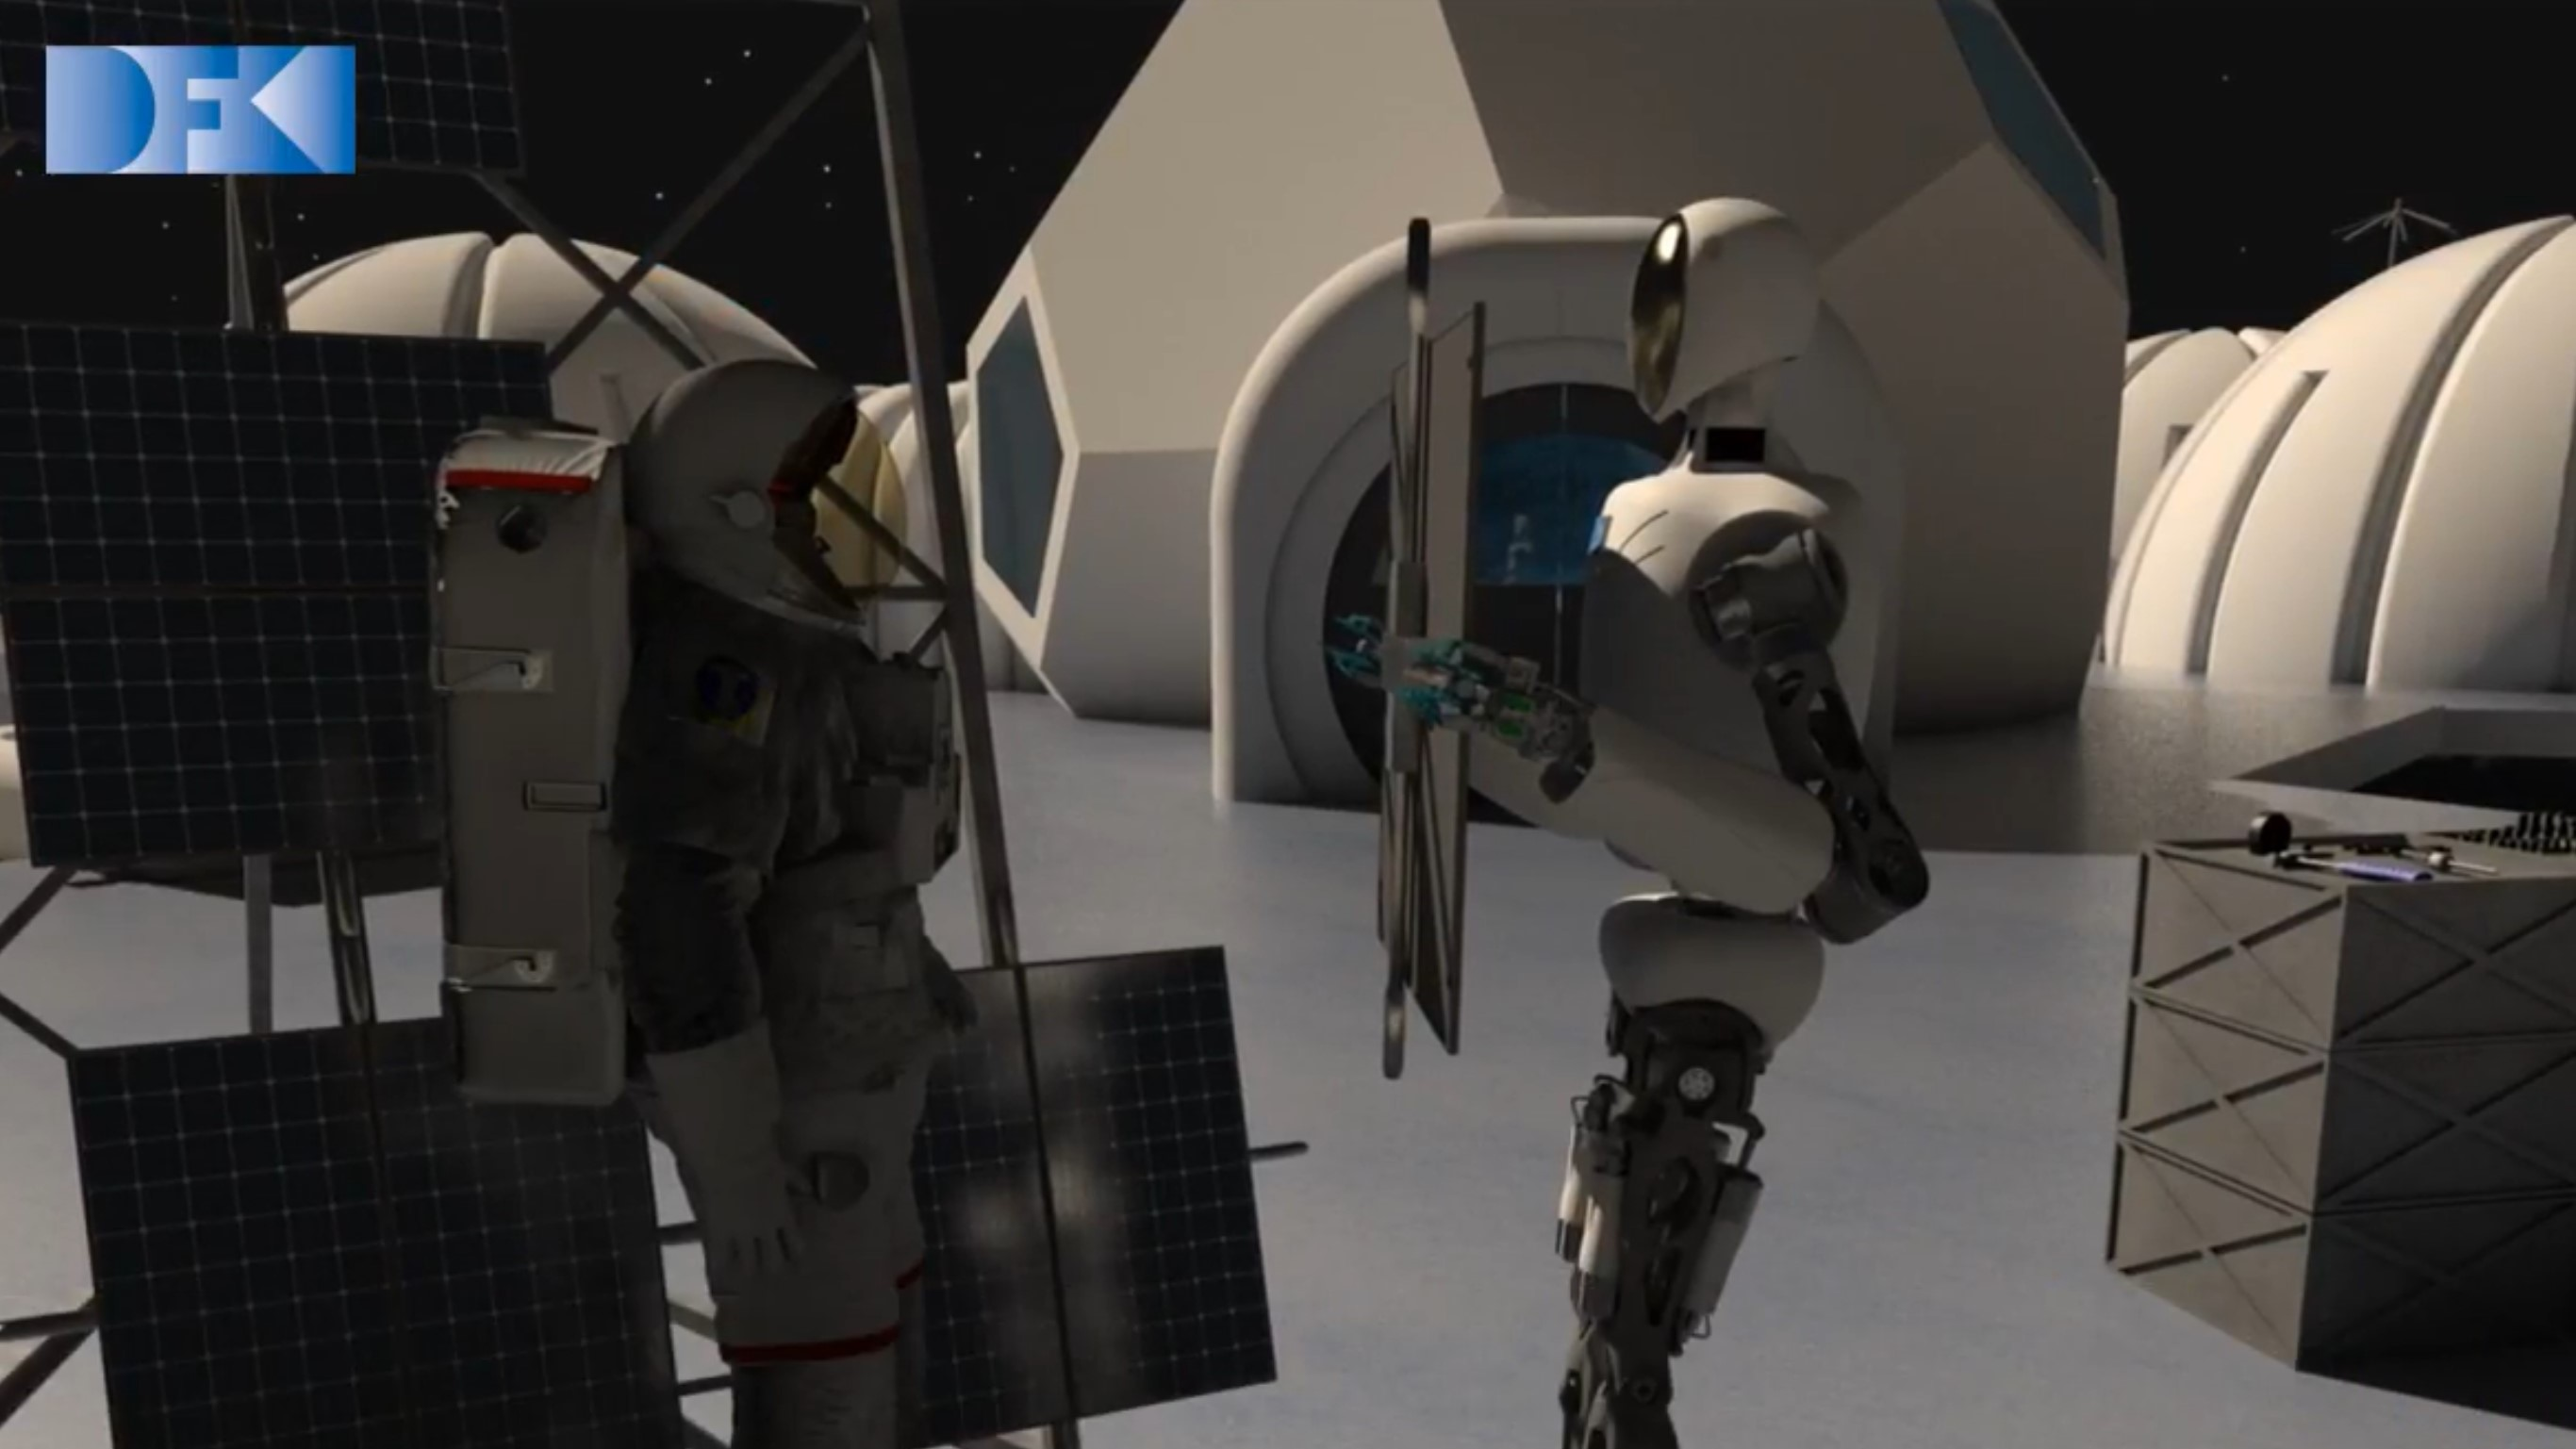
\includegraphics[width=.7\textwidth]{img/rh5_interactive_16_9.jpg}
\caption{Humanoid robots can interact with humans in a very intuitive manner since they share similar kinematics, sensing and behavior. This opens up new opportunities for the cooperation needed, e.g. when assembling and installing infrastructure on foreign planets \cite{img:rh5_interactive}.}
\label{img:rh5_interactive}
\end{figure} 
    
We perform all these tasks seemingly effortless. But compared to current robots, the dynamic capabilities of humans and animals are still outstanding in terms of versatility, speed, efficiency and robustness \cite{hutter2012starleth}. In order to further close the gap between robots and their natural counterparts, current research is driving towards exploiting the natural dynamics of robots. This implies mutually dependent changes about how we think about the robots design \cite{pratt2004series} on the one hand and about ways of controlling them on the other hand, in order to move in a more dynamic, efficient and natural way \cite{collins2005efficient, haddadin2012optimal, pratt2000exploiting}.
%\begin{figure}[t]
%	\begin{subfigure}{.5\textwidth}
%		\centering
%		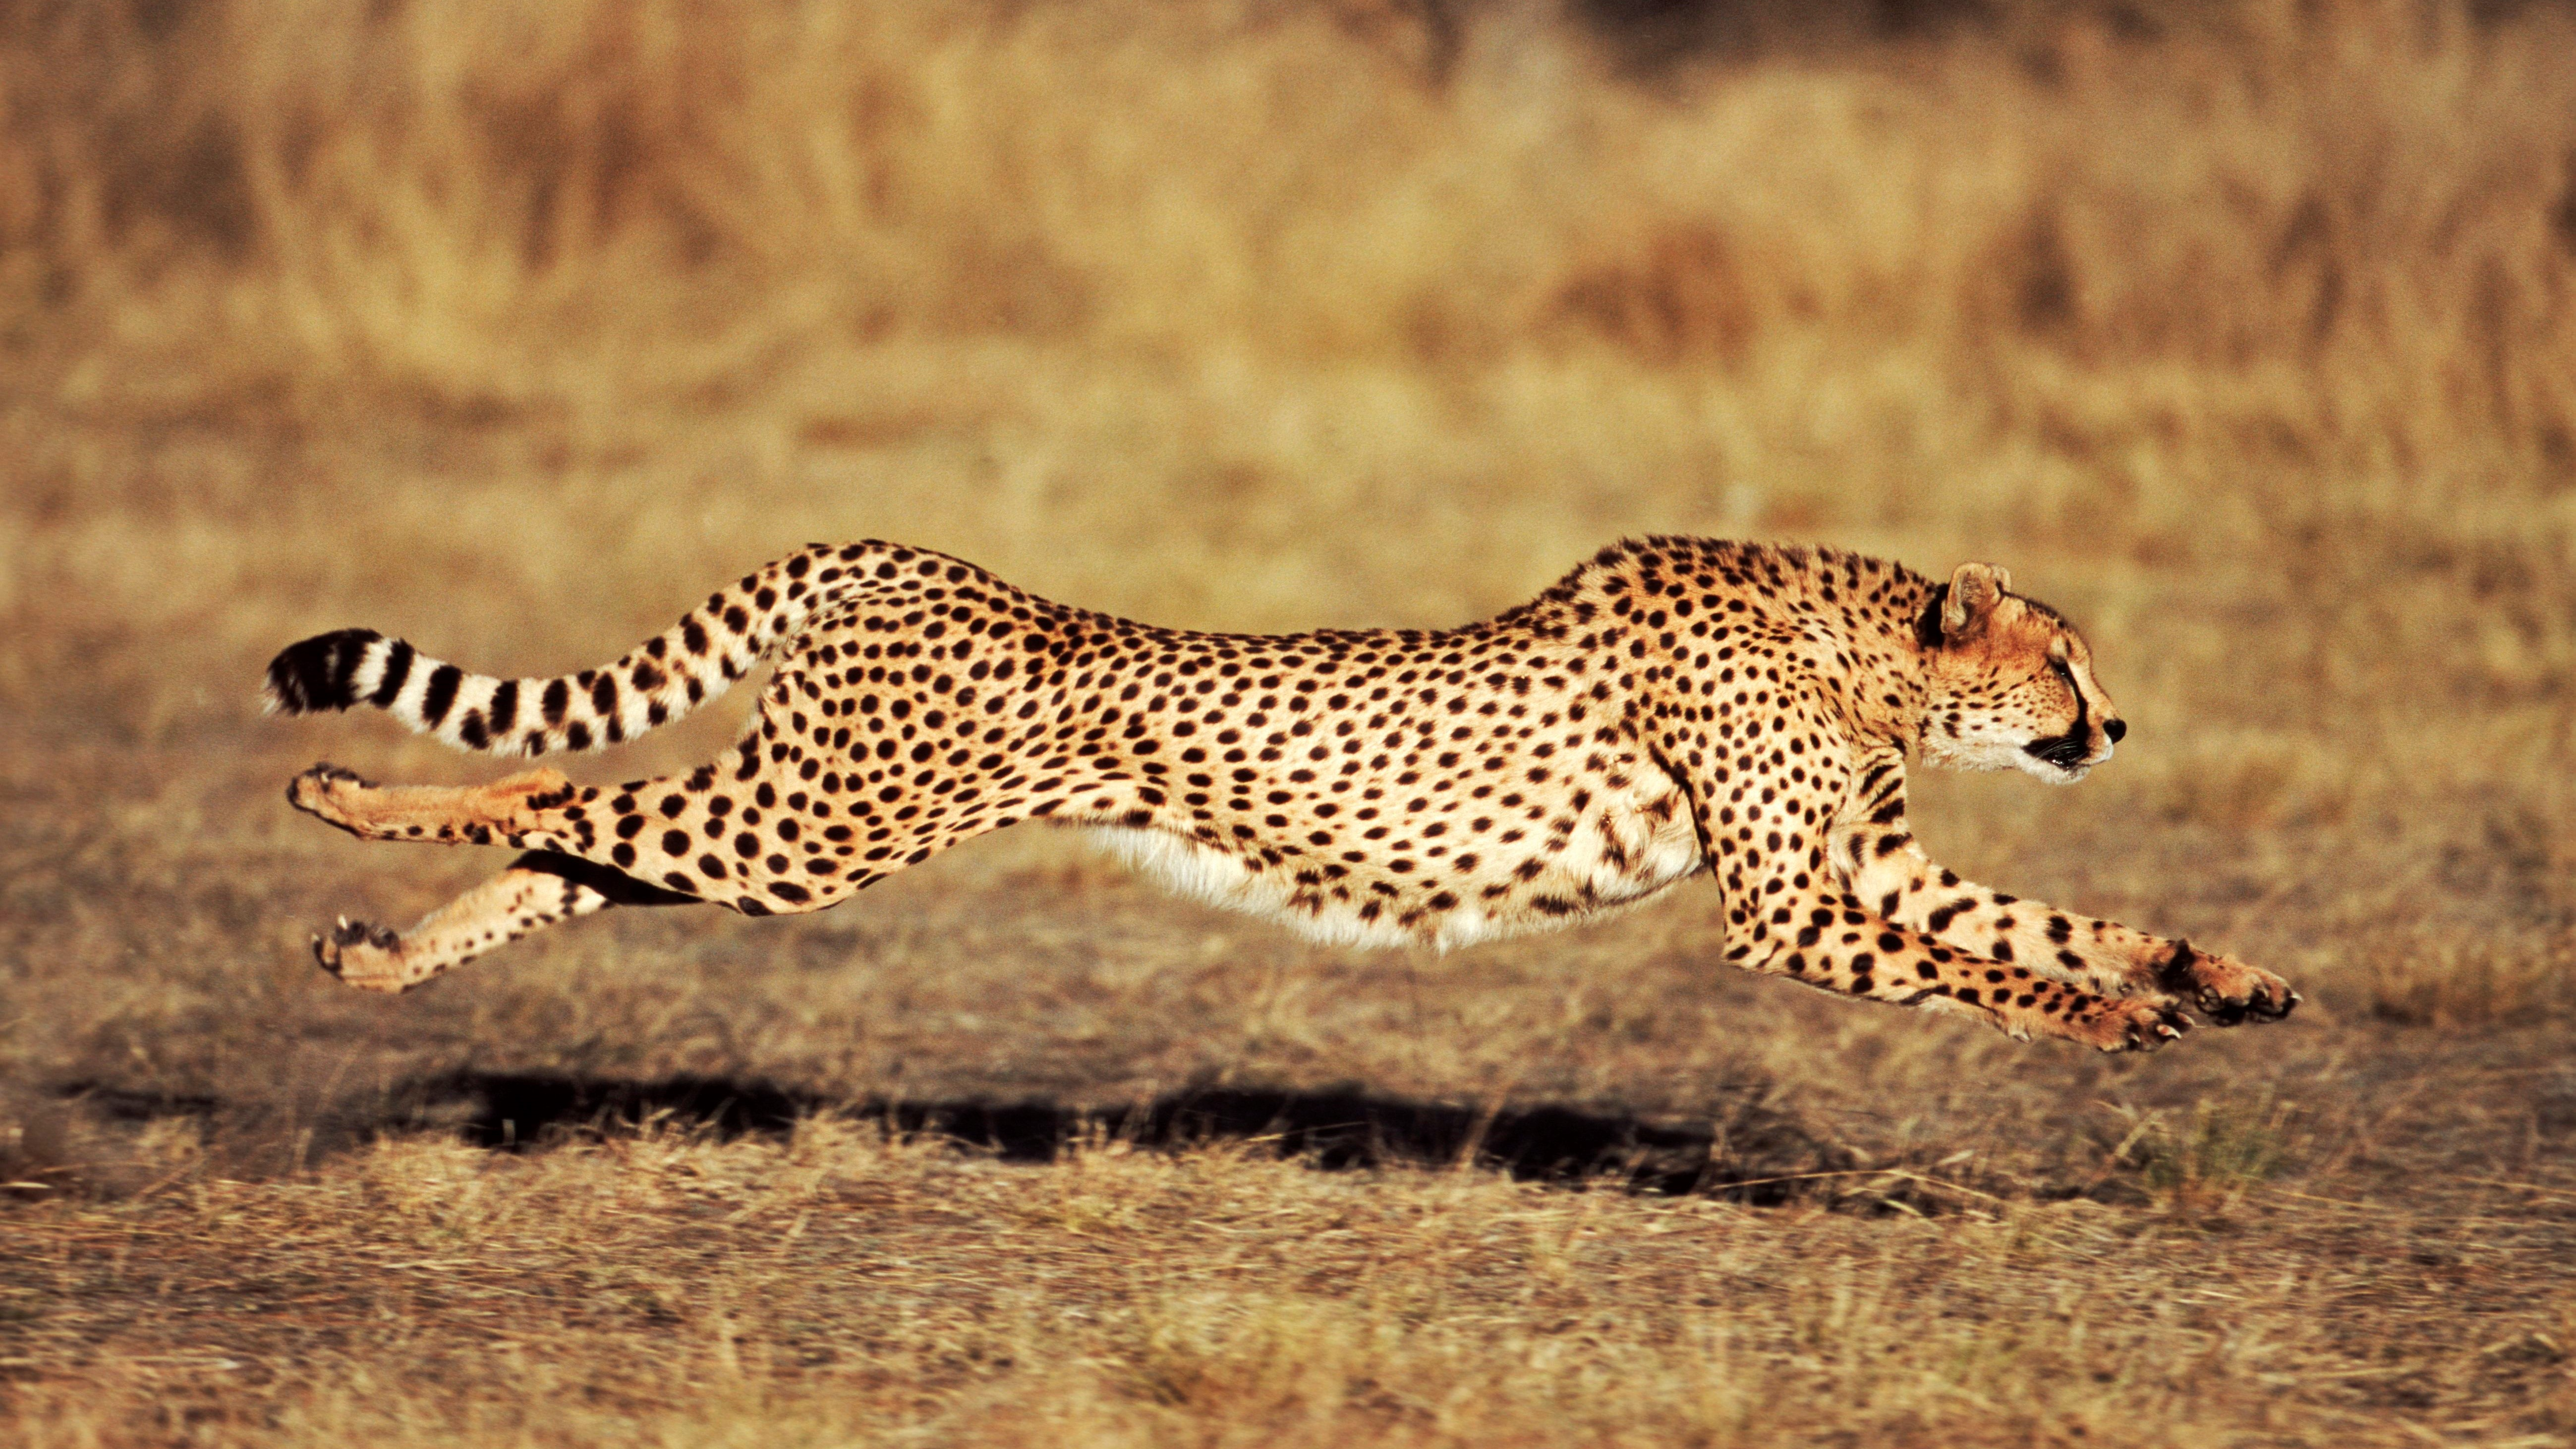
\includegraphics[width=.95\linewidth]{img/cheetah_run_16_9}
%		\caption{Animal in dynamic movement \cite{img:cheetah_run}}
%		\label{fig:animal}
%	\end{subfigure}%
%	\begin{subfigure}{.5\textwidth}
%		\centering
%		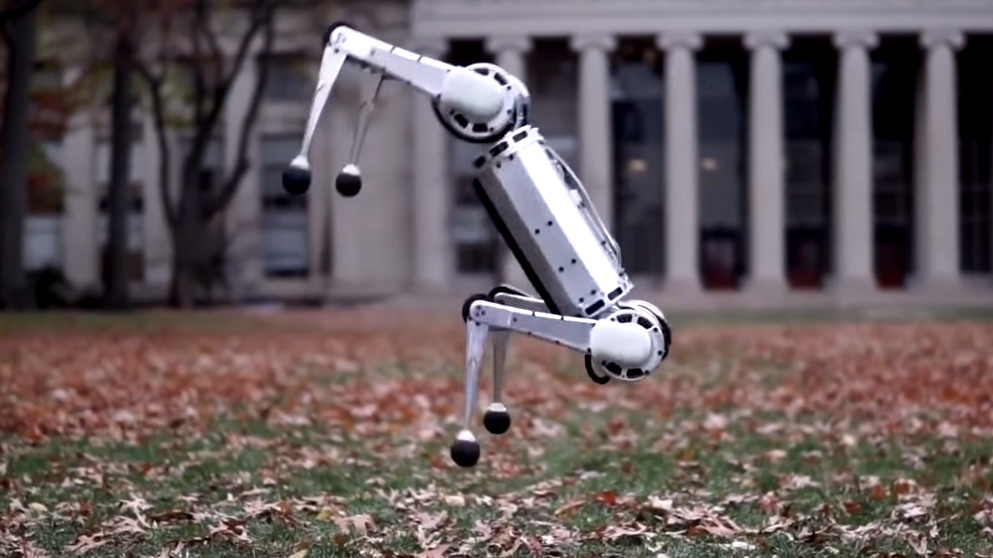
\includegraphics[width=.95\linewidth]{img/mini_cheetah_16_9}
%		\caption{Quadruped Robot Mini Cheetah \cite{img:mini_cheetah}}
%		\label{fig:bert}
%	\end{subfigure}
%	\caption[Quadrupedal locomotion of robots and their biological counterparts.]{Animals and humans combine versatility, speed robustness and efficiency in perfection when moving in rough terrain (a). While important issues in making legged robots (b) move performantly already have been addressed, energy efficiency is one of the major drawbacks in comparison to their biological counterparts.}
%	\label{fig:natural2robot}
%\end{figure}

The specific difficulty of creating bipedal walking motions has several causes. The first difficulty is due to the mechanism complexity, i.e. dealing with high-dimensional degrees of freedom, leading to potentially expensive computations. Secondly, legged locomotion is subject to different contact and impact collisions, resulting in multi-phase models and hence hybrid dynamics. Finally, bipeds face the problem of effective underactuation, further restricting the applicable control approaches.

\textit{Dynamic} bipedal locomotion adds additional complexity to this problem. A central characteristic of walking dynamically is that the center of mass (COM) partially leaves the biped's support polygon. Furthermore there is the need of generating feasible, controllable limit cycles. When considering running motions, difficulties are faced regarding the conservation of angular momentum, which implies restrictions on the controllability during flight phases \cite{westervelt2018feedback}. 


\section{Related Work}
There are existing numerous ways to generate feasible motion plans for robotic systems. Common approaches are relying on simplified dynamic models, while recent ones make use of numerical optimization for generating efficient motion plans. 

\subsection{Traditional Legged Locomotion Planning}
Previously we have already seen, why locomotion synthesis for legged robots is a challenging problem. Solving this global problem typically is approached by splitting it up into successive subproblems that are solved sequentially: (i) Contact planner, (ii) Centroidal pattern generator, (iii) Whole-body motion generator (\cref{img:traditional_locomotion_planner}) \cite{carpentier2017multi}. 
\begin{figure}[h!]
\centering	
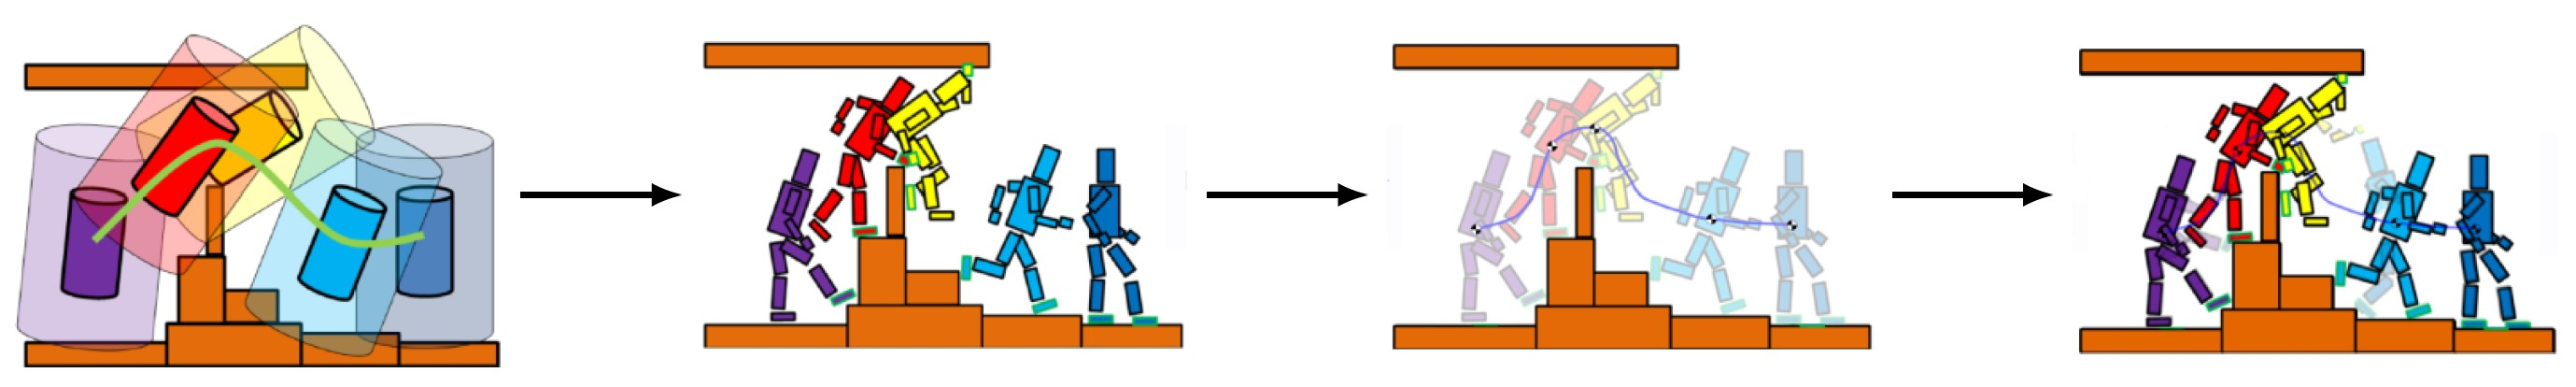
\includegraphics[width=1\textwidth]{img/traditional_locomotion_planner.jpg}
\caption{Tradional Legged Locomotion Planning \cite{giraud2020motion}.}
\label{img:traditional_locomotion_planner}
\end{figure}  
The first stage of traditional legged locomotion planning is a contact planner that selects appropriate foothold position and step timings. In other words, this component predefines \textit{where} and \textit{when} external forces can act on the system. 
Once these force locations have been predetermined, the goal is to generate a body motion, i.e. a \gls{CoM} and end-effector trajectories, which can be created with the available forces. A common approach is to model the robot as a \gls{LIP} and find a motion where the \gls{CoP} remains inside the \gls{SP}. The \gls{LIP} can be solved analytically and efficiently and consequently has been used in a variety of approaches \cite{kajita2003biped, kalakrishnan2010fast, winkler2015planning, bellicoso2017dynamic}. 
From the contact sequence and the centroidal trajectory, a dynamic-physical whole-body trajectory has to be found. This often is done by solving the \gls{IK} \cite{espiau1992new} or operational-space \gls{ID} \cite{khatib1987unified} of the system and produces appropriate joint positions or torques, respectively that can be applied to a physical system.

This approach is beneficial in terms of computation time but comes at the cost of limited motion complexity and energy efficiency. 
The first limitation comes from the underlying assumptions of the \gls{LIP} model. More complex motions and terrains might require to place feet at different heights, reorientation of the base or jump vertically \cite{winkler2018optimization}. Another limitation arises from the fact whole-body planning produces more efficient motions than a simple program such as an \gls{IK} solver \cite{budhiraja2018differential}.   

\subsection{Trajectory Optimization}
Generating motion plans for dynamic systems is subject to \gls{TO} algorithms that belong to the broader research field of \gls{OC}. 

\gls{TO} is a numerical optimization technique with the goal of finding a state-control sequence, which locally minimizes a predefined cost function given a set of constraints. The approach allows to specify the behavior of a robot directly in the task space, e.g. a desired end-effector trajectory, while reducing the amount of hand-crafted components. 

There are existing different methods to formulate a \gls{TO}, namely \textit{direct} and \textit{indirect} methods. Unlike \textit{direct} methods which explicitly represent the state, \textit{indirect} methods only represent the controls while the state is obtained from forward simulation of the system. In direct methods, the \gls{OC} problem is transcribed into a \gls{SQP}, which easily handles both equality and inequality constraints and is implemented in generic off-the-shelf solvers. Consequently, the direct approaches are forced to search in a constrained optimization space which is slower but finds better optima. The indirect approaches are more sensitive to local minima, but are faster and better suited for warm-starting. For a comprehensive overview and further information on \gls{TO} methods see \cite{betts1998survey, kelly2017transcription, tassa2014control}.

\gls{TO} based on reduced centroidal dynamics \cite{orin2013centroidal} has become a popular approach in the legged robotics community. In some approaches it is used after planning the contacts \cite{dai2014whole, carpentier2016versatile, herzog2015trajectory} while other approaches simultaneously optimize the centroidal trajectory and the contacts \cite{mastalli2017trajectory, winkler2018gait, aceituno2017simultaneous}. Either way, the transfer from centroidal to whole-body dynamics is only achieved by instantaneous feedback linearization where typically quadratic programs with task-space dynamics are solved \cite{saab2013dynamic, herzog2016momentum, vaillant2016multi}. 

While \gls{TO} based on reduced dynamics models has shown great experimental results, whole-body \gls{TO} instead is proven to produce more efficient motions, with lower forces and impacts \cite{budhiraja2018differential}. Hence we will focus on \textit{indirect methods}, namely \gls{DDP} to compute the whole-body motion. \gls{DDP} allows to efficiently solve nonlinear \gls{OC} problems due to its intrinsic sparse structure and is introduced in \crefrange{sec:TheoryDDP}{sec:TheoryConstrainedDDP} in more detail.

\subsection{Crocoddyl Framework} 
Crocoddyl (Contact RObot COntrol by Differential DY1namic Library) is a recently presented open-source framework for efficient multi-contact optimal control \cite{mastalli20crocoddyl}, which is used within this thesis to plan whole-body motions. 

The framework allows to efficiently compute optimal robot trajectories with pre-defined contact phases. Its solver is based on various efficient \gls{DDP}-like algorithms. Along with the Crocoddyl, a novel optimal control algorithm called \gls{FDDP} is introduced. The \gls{FDDP} algorithm is an improved version of the classical \gls{DDP} algorithm, which shows a greater globalization strategy due to two modifications. First, the backward pass also allows for infeasible state and control trajectories. Second, forward pass keeps the gaps open within the first iterations. 
The framework can be used in one of two ways: Either offline, where a stabilizing controller is build around the nominal trajectory \cite{giraud2020motion} or in a \gls{MPC} sense, where the optimal trajectory is (re-)computed online. 

Crocoddyl allows the computation of highly-dynamic movements (e.g. jumping, front-flip) within few milliseconds. However, these exemplary case studies do not guarantee inherent balance of the motions, leading to trajectories that are hard to stabilize on a real system. To this end, we present a generic method for constraining DDP-like solvers in order to generate inherently balanced, dynamic motions that are applicable on real robots.    

\subsection{RH5 Humanoid Robot}
The derived motion planning approach has been tested both in simulation and real-world experiments on a full-size humanoid robot. RH5 is a lightweight and biologically inspired humanoid that has recently been developed at DFKI Robotics Innovation Center \cite{peters2017konstruktion}.

The RH5 humanoid robot (see \cref{img:rh5_robot}) is designed to mimic the human anatomy with a total size of 200cm, a weight of 62kg and a total of 32 \gls{DoF}. The two legs account for 12 \gls{DoF}, the torso and neck kinematics each for three and the arms and grippers of the robot for 14 \gls{DoF}. In order to achieve a high dynamic performance, the robot's design follows a series-parallel hybrid approach. Consequently,linkages and parallel mechanisms are utilized in most of the robots joints, e.g. the hip-flexion-extension, knee, ankle, torso and wrist. A comparison of RH5 with other state of the art humanoid robots revealed several advantages of this design approach, including better maximum velocity and torque of the ankle as well as an advantageous weight of the lower leg \cite{kumar2020survey}. The interested reader can find a comprehensive introduction on series-parallel hybrid robots in \cite[Ch.2]{kumar2019modular}. 

\begin{figure}[h!]
\centering	
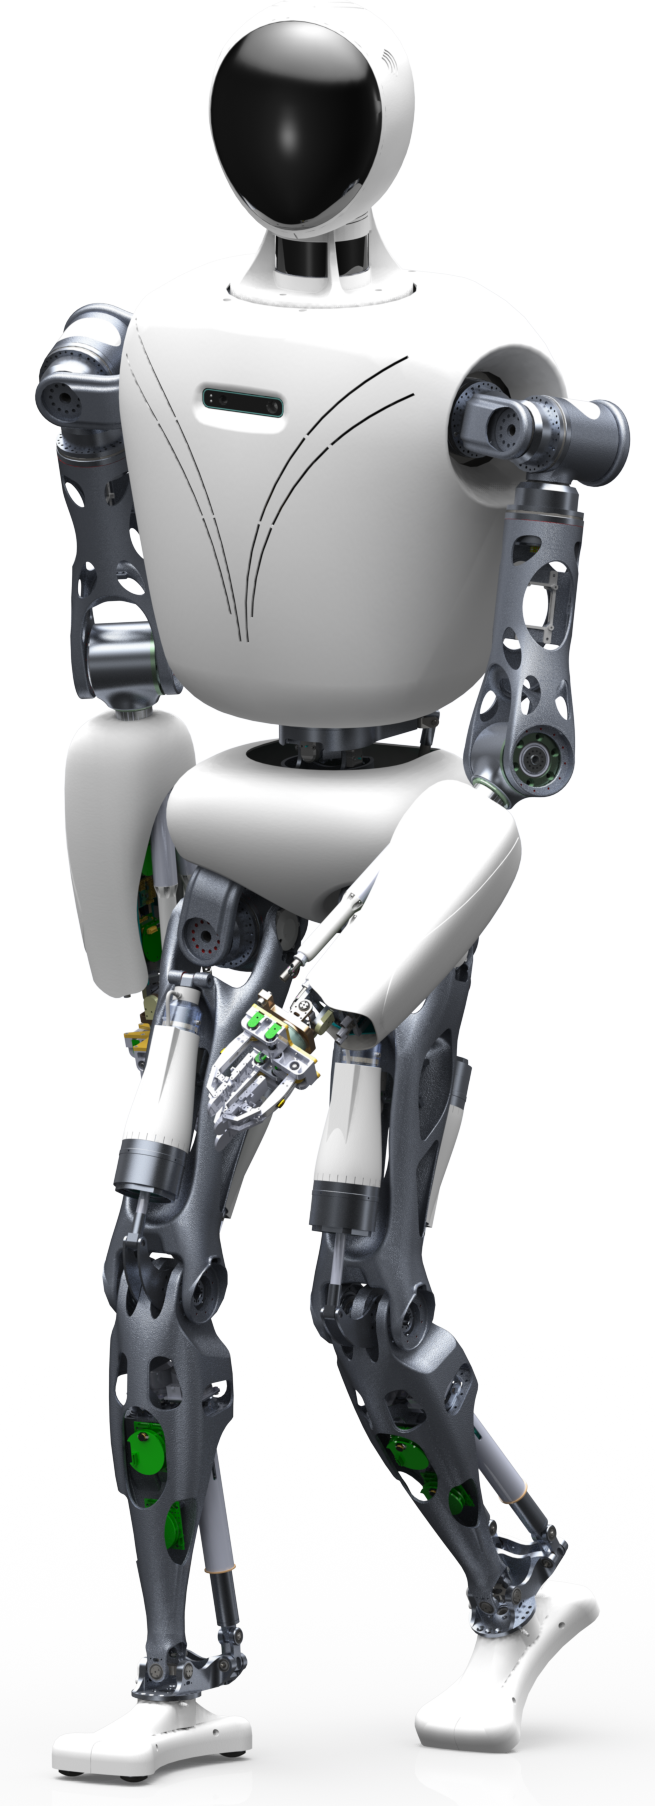
\includegraphics[width=.2\textwidth]{img/rh5_robot}
\caption{The recently presented RH5 is a lightweight and biologically inspired humanoid used as experimental platform within this thesis.}
\label{img:rh5_robot}
\end{figure} 


\section{Contributions}
The overall goal of this master's thesis is to contribute to the research field of humanoid robotics by applying, evaluating and extending recently presented whole-body \gls{TO} approaches on the RH5 humanoid robot. 

The proposed motion planning approach (see \cref{img:approach}) consists of a DDP-based whole-body \gls{TO}. 
Beneath the contact position and timings, it also considers a set of contact stability constraints that allow computing inherently balanced motions. In contrast to many other motion planning concepts followed by the legged robotics community, our approach (i) considers the full robot dynamics instead of using a reduced dynamics model such as the \gls{LIP} model (ii) simultaneously optimizes for the centroidal motion, contact stability and whole-body trajectory instead of a sequential optimization. The specific contributions of this thesis are summarized below.
\begin{figure}[h!]
\centering	
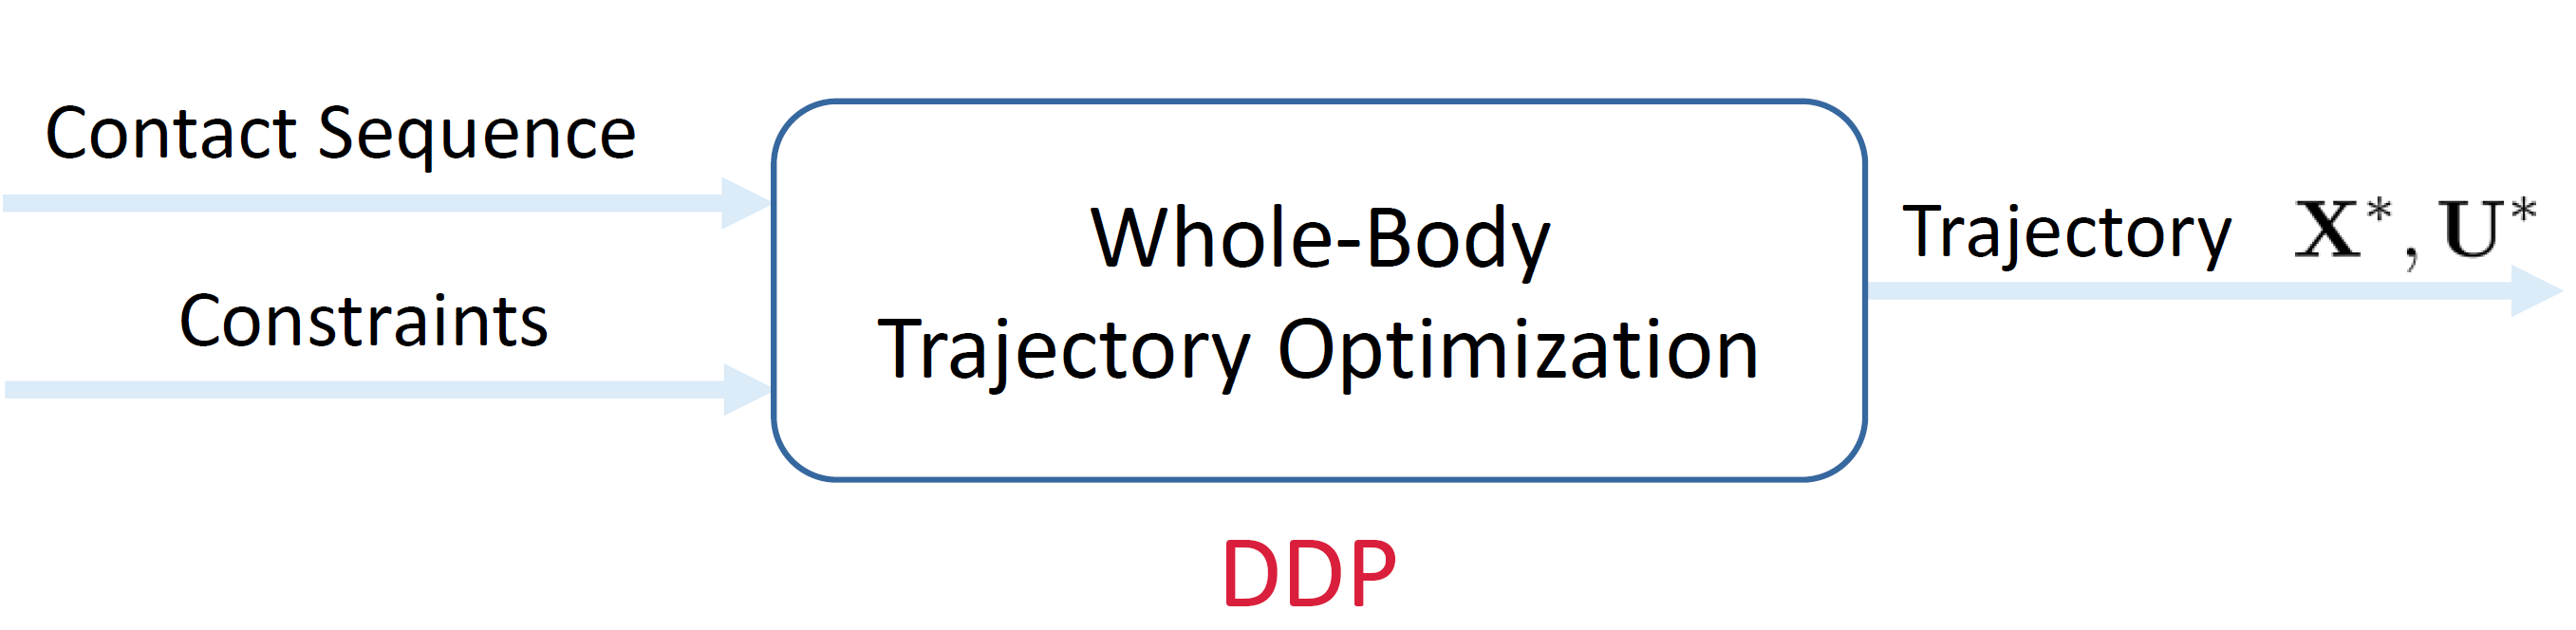
\includegraphics[width=.8\textwidth]{img/approach}
\caption{The motion planning approach proposed within this thesis. Based on predefined foothold positions, step timings and stability constraints a \gls{DDP}-based whole-body \gls{TO} is used to generate inherently balanced motions plans.}
\label{img:approach}
\end{figure}

\paragraph{C1.} A generic method for constraining DDP-like solvers in order to generate inherently balanced dynamic motions. The results are integrated into the open-source framework Crocoddyl.
\paragraph{C2.} Evaluation of the stability of the proposed motion planning approach for bipedal walking gaits of increasing complexity in simulation. 
\paragraph{C3.} Identification of range of motions for the RH5 humanoid by performing highly-dynamic movements as basis for future design iterations. 
\paragraph{C4.} An experimental pipeline for executing optimization-based whole-body motions on a series-parallel hybrid robot.   


\section{Structure}
This thesis is organized in a total of 8 chapters. Fig. XXX shows the overall outline of this thesis. In the following, a summary of each chapter is provided which allows the readers to easily navigate through this document.
\paragraph{Chapter 1 (Introduction)} motivates the problem and presents the related work and specific contributions. It also provides details on the structure of the thesis.
\paragraph{Chapter 2 (Mathematical Background)} provides the reader with fundamental background in bipedal locomotion and stability analysis. Furthermore, it introduces the class of algorithms and relevant extensions used in this work.
\paragraph{Chapter 3 (Contact Stability Constrained DDP)} presents a generic method for integrating stability constraints into DDP-like solvers in order to generate inherently balanced dynamic motions.
\paragraph{Chapter 4 (Bipedal Walking Variants)} studies the proposed motion planning approach for bipedal walking gaits of increasing complexity in simulation.
\paragraph{Chapter 5 (Highly-Dynamic Movements)} presents an analysis of highly-dynamic movements based on the proposed motion planning approach with the goal of identifying the system limits of the RH5 humanoid robot. 
\paragraph{Chapter 6 (Validation in Real-Time Physics Simulation)} presents a validation of the generated motions by application of a simple control architecture in an real-time physics simulation environment. 
\paragraph{Chapter 7 (Validation in Real-World Experiments)} presents an experimental pipeline for validating the motions on a full-size humanoid robot with series-parallel hybrid mechanisms. 
\paragraph{Chapter 8 (Conclusion and Outlook)} presents the summary of the thesis and identifies future research directions. 


